\section{Introducción}
% Especificar la motivación y las características principales del proyecto como así también un marco general
% sobre el estado del arte de la tecnología y el uso de las ideas o conceptos del proyecto propuesto.
En el ámbito universitario resulta necesario mantener informadas a las personas sobre una amplia variedad de hechos, noticias y acontecimientos que sucedieron o sucederán, desde la ubicación de un aula hasta la notificación de la cancelación de una clase. Muchas veces estas notificaciones son sobre cuestiones muy efímeras, lo que requiere rapidez para empezar a transmitirlas y facilidad para tener el alcance necesario.

En las facultades de la Universidad Nacional de La Plata se consumen muchos recursos para cumplir este fin, a través de afiches, pancartas, panfletos, etc. los cuales, pese a ser de barata fabricación, no tienen una vida útil muy extensa. Además todas estas formas de comunicacion se basan en el uso de papel, que tras ser utilizado debe desecharse debido a la imposibilidad de reutilizarlo, generando una cantidad de residuos significativa. Si se tiene en cuenta que también generan una polución visual considerable, por la gran cantidad de estos distribuidos en todos los lugares transitables, resulta prudente considerar una nueva forma de comunicación.

Surge así la idea de desarrollar de un cartel electrónico reutilizable, capaz de ser configurado remotamente por las autoridades competentes, con el fin de proveer una forma de comunicación masiva más limpia, clara y menos dañina para el medio ambiente. 

\section{Objetivos del proyecto}
% Deben especificarse los objetivos que se plantearon en el informe inicial
% (primarios y secundarios) se hayan cumplido o no (en las conclusiones se deberá contemplar
% el cambio de objetivos o el grado de cumplimiento de los mismos).
El objetivo principal del proyecto es implementar un cartel de LEDs que pueda ser configurado remotamente por un usuario.
El mismo se puede subdividir en subobjetivos, los cuales se mencionan a continuación:

Diseñar e implementar el Hardware (PCB, matrices de LEDs) del cartel para que visualice correctamente el mensaje configurado. Deberá ser modular, es decir, que sea posible agregar letras, expandiendo la cantidad de caracteres en un renglón.

Desarrollar el software embebido que se ejecutará en el microcontrolador.

Desarrollar el software que controla el cartel. Éste podrá ser usado desde una PC y tendrá una interfaz gráfica con formato de panel para controlar las características del mensaje a mostrar por el cartel.

Diseñar e implementar protocolo de comunicación para la comunicación entre el software controlador del panel y el cartel. El protocolo debe establecer un método de autenticación que impida el acceso de personal no autorizado al cartel. Esto implica que sea seguro antes ataque del tipo \emph{man-in-the-middle} y otros tipos de ataques bien conocidos.

\section{Diseño del hardware}
% Describir el hardware propuesto, comenzando por un diagrama en bloques, luego una descripción de las Interfaces eléctricas
% (conexiones poncho-EDU-CIAA) y de usuario (teclado, displays, etc)
% hasta llegar al detalle fino de los componentes y circuitos a utilizar y sus características.
El hardware está compuesto por módulos. Cada módulo puede encargarse o bien de la lógica o bien de la adaptación de la misma a la visualización del mensaje, según el tipo de módulo. Los módulos están armados con matrices de LEDs de 8x8, chips controladores \cite{MAX7219} encargados de actualizar el estado de cada LED en función del caracter mostrado y componentes pasivos varios (ver figura \ref{fig:hw-moduloEsquematico}). 

Hay dos tipos de módulos: un maestro y un esclavo. El módulo maestro cuenta con un microcontrolador, reguladores de tensión, un conector expuesto al usuario y teclas de reset de comunicación (reinicia la configuracion Wi-Fi) y de alimentación (reinicia la alimentación del microcontrolador). Un solo módulo maestro puede controlar N módulos esclavos. Se puede observar su circuito en la figura \ref{fig:master}.

\begin{figure}[ht!]
	\begin{center}
		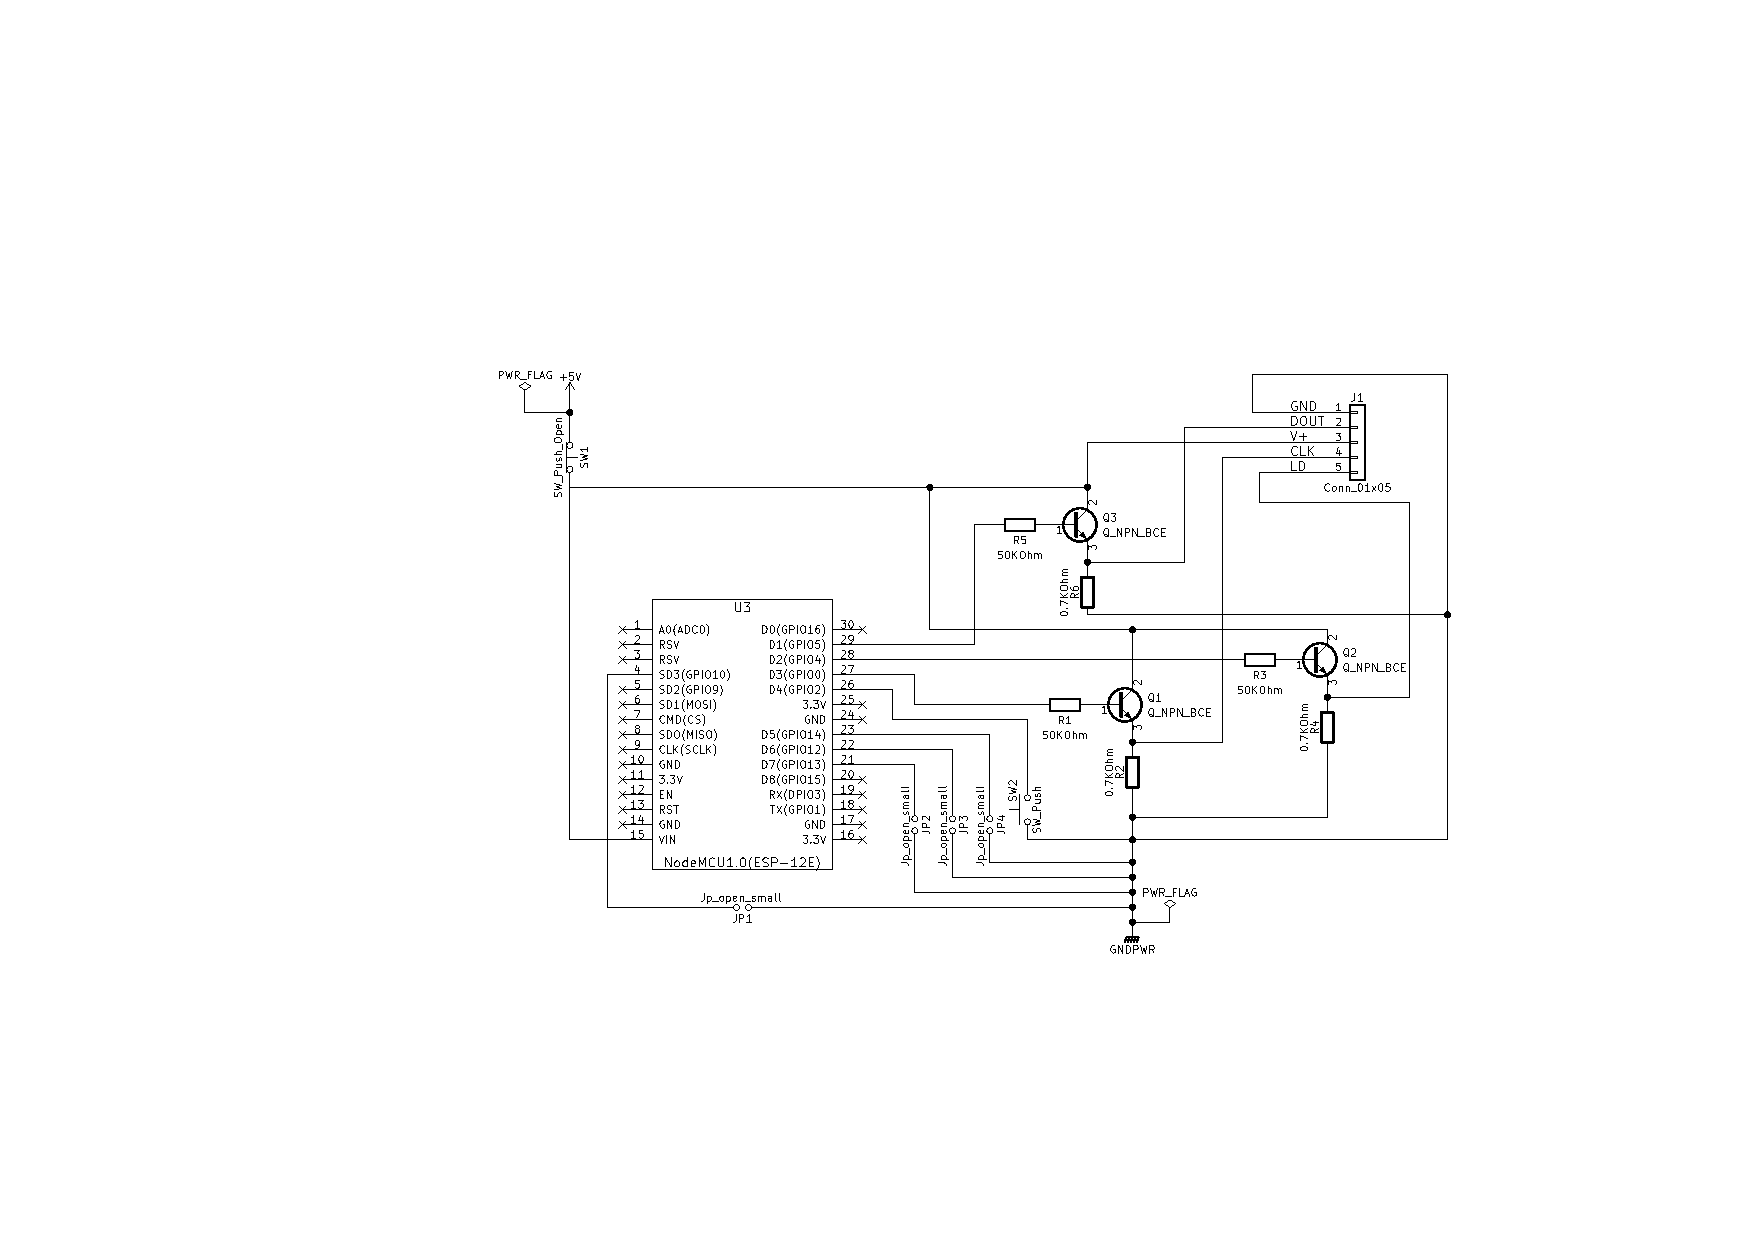
\includegraphics[scale=0.8]{imagenes/hw/master.pdf}
		\caption{Circuito del módulo maestro}
		\label{fig:master}
	\end{center}
\end{figure}

Los módulos esclavos no llevan microcontrolador, sino que en cambio cuentan con dos conectores (uno de entrada y uno de salida) para poder conectar secuencialmente varios esclavos en \emph{daisy-chain}, como se ilustra en la figura \ref{fig:esquema-general}. Dichos conectores transmiten la alimentación y las señales necesarias para la emisión sincronizada del mensaje entre todos los esclavos. La totalidad de los componentes del módulo puede verse en la figura \ref{fig:slave}.

\begin{figure}[ht!]
	\begin{center}
		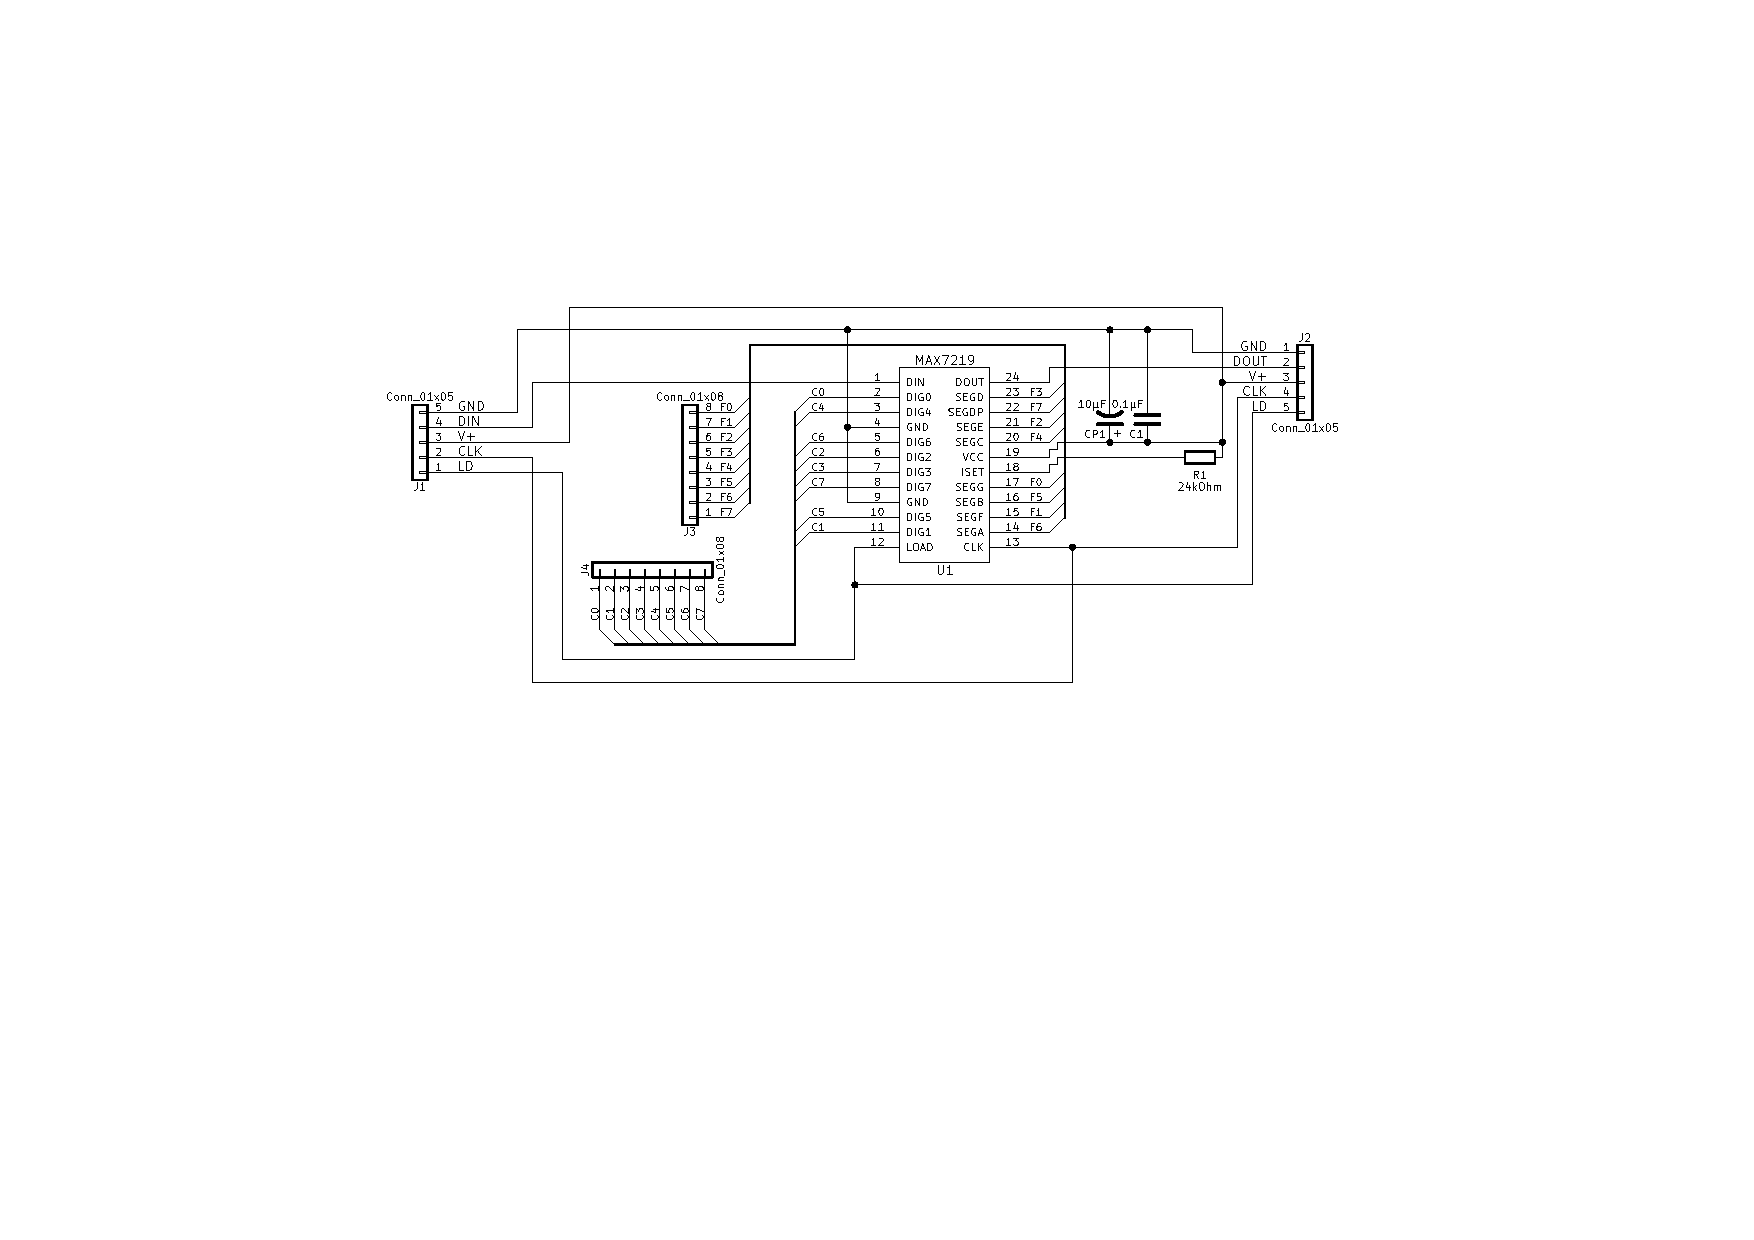
\includegraphics[scale=0.8]{imagenes/hw/slave.pdf}
		\caption{Circuito del módulo esclavo}
		\label{fig:slave}
	\end{center}
\end{figure}

Uno de los factores que limitarán la cantidad máxima de módulos esclavos que se pueden conectar será la corriente máxima que puede entregar la fuente de tensión y el regulador que se utilice en el módulo maestro.

\begin{figure}[ht!]
	\begin{center}
		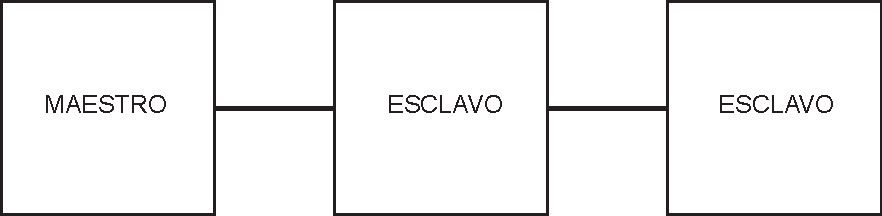
\includegraphics[scale=0.8]{imagenes/hw/esquema-general.pdf}
		\caption{Esquema general del sistema}
		\label{fig:esquema-general}
	\end{center}
\end{figure}

\subsection{Controlador}
Como controlador principal se usará el kit de desarrollo NodeMCU, que integra un AI-Thinker ESP-12E (figura \ref{fig:foto-esp12e}), el cual contiene un SoC (\emph{System on Chip}) ESP8266EX (figura \ref{fig:esp8266ex}) de la empresa Espressif. El módulo NodeMCU es hardware libre, sin embargo, el ESP12E y el ESP8266EX no lo son.\cite{NodeMCU}

\begin{figure}[ht!]
	\begin{center}
		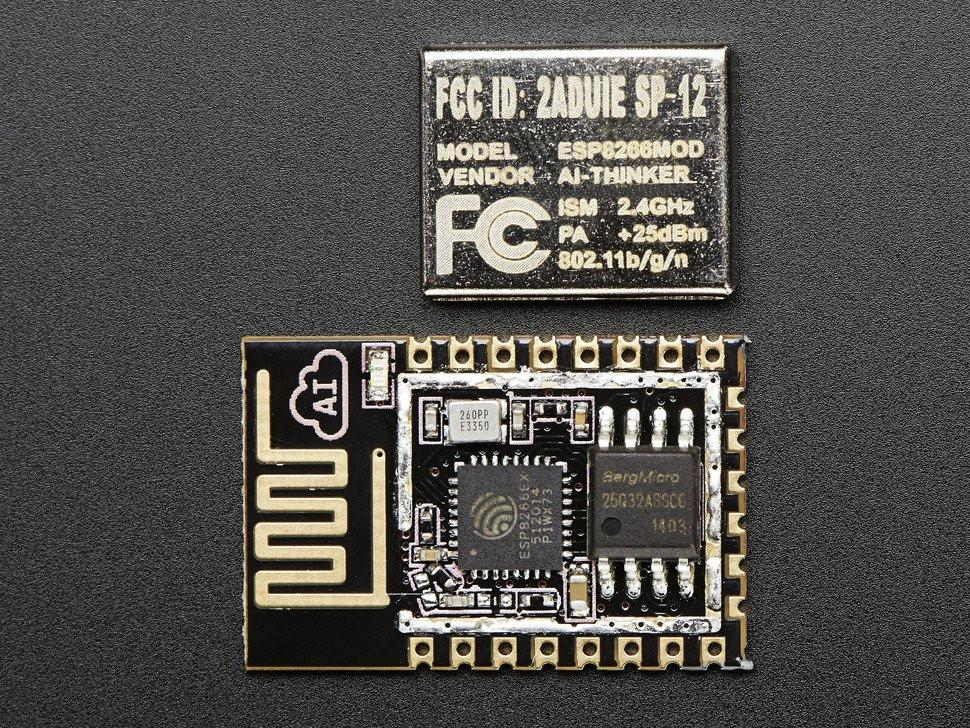
\includegraphics[width=8cm]{imagenes/esp12e-foto.jpg}
		\caption{Foto del módulo ESP12E sin su cubrimiento.}
		\label{fig:foto-esp12e}
	\end{center}
\end{figure}

\begin{figure}[ht!]
	\begin{center}
		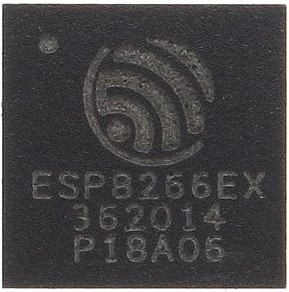
\includegraphics[width=3cm]{imagenes/esp8266ex.jpg}
		\caption{Foto del integrado ESP8266EX.}
		\label{fig:esp8266ex}
	\end{center}
\end{figure}

\begin{figure}[ht!]
	\begin{center}
		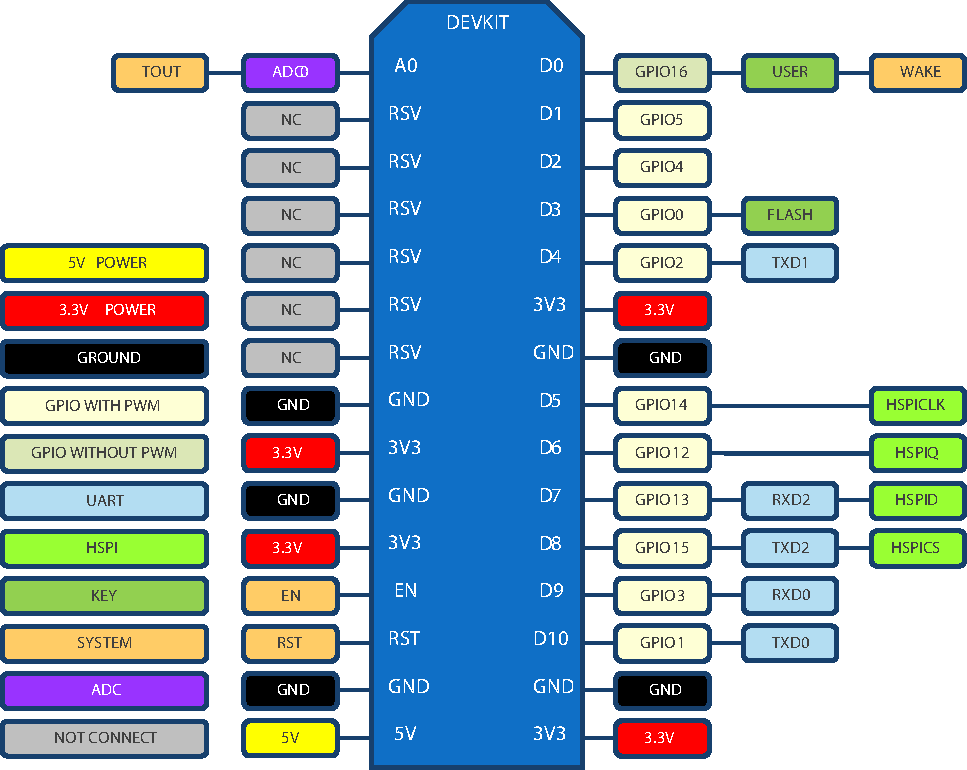
\includegraphics[width=12cm]{imagenes/nodemcu-pinout.pdf}
		\caption{Asignación de pines del NodeMCU.}
		\label{fig:nodemcu-pinout}
	\end{center}
\end{figure}

Es importante tener en cuenta que el sistema no integra en su hardware directamente ni el ESP12E ni el ESP8266EX, sino que integra el NodeMCU, cuya asignación de pines se puede ver en la figura \ref{fig:nodemcu-pinout}.

El chip ESP8266EX combina un microcontrolador Tensillica Xtensa L106, un RISC de 32 bits corriendo a 80 Mhz, con funcionalidad WiFi. \cite{ESP8266Datasheet} El chip tiene memoria ROM con firmware no removible, y puede correr programas almacenados en flash externa. Para poder usar todas sus funcionalidades, se debe programar sobre firmware privativo desarrollado por Espressif, esto implica que el programa de usuario corre en simultáneo con el firmware y el uso de la memoria de trabajo está sujeto a la versión del firmware. Según el datasheet, el usuario puede esperar tener disponible 50 KiB de SRAM.

Como se mencionó anteriormente, se necesita de flash externa para correr programas. El módulo ESP-12S se encarga de proveer al ESP8266EX 4 MiB de memoria flash.

\subsection{Módulos}
El cartel se compone de módulos: un maestro y esclavos. Cada módulo esclavo contiene una matriz de LED 8x8, un chip controlador \cite{MAX7219} y componentes pasivos varios (ver figuras \ref{fig:hw-moduloEsquematico} y \ref{fig:hw-moduloLED}). A diferencia de los módulos esclavo, el módulo maestro posee un microcontrolador NodeMCU que recibe los pedidos del usuario (ver figura \ref{fig:hw-diagrama-general}), procesa la información codificando los caracteres y transmite dichos datos a los esclavos conectados para que muestren la información.

\begin{figure}[ht!]
	\begin{center}
		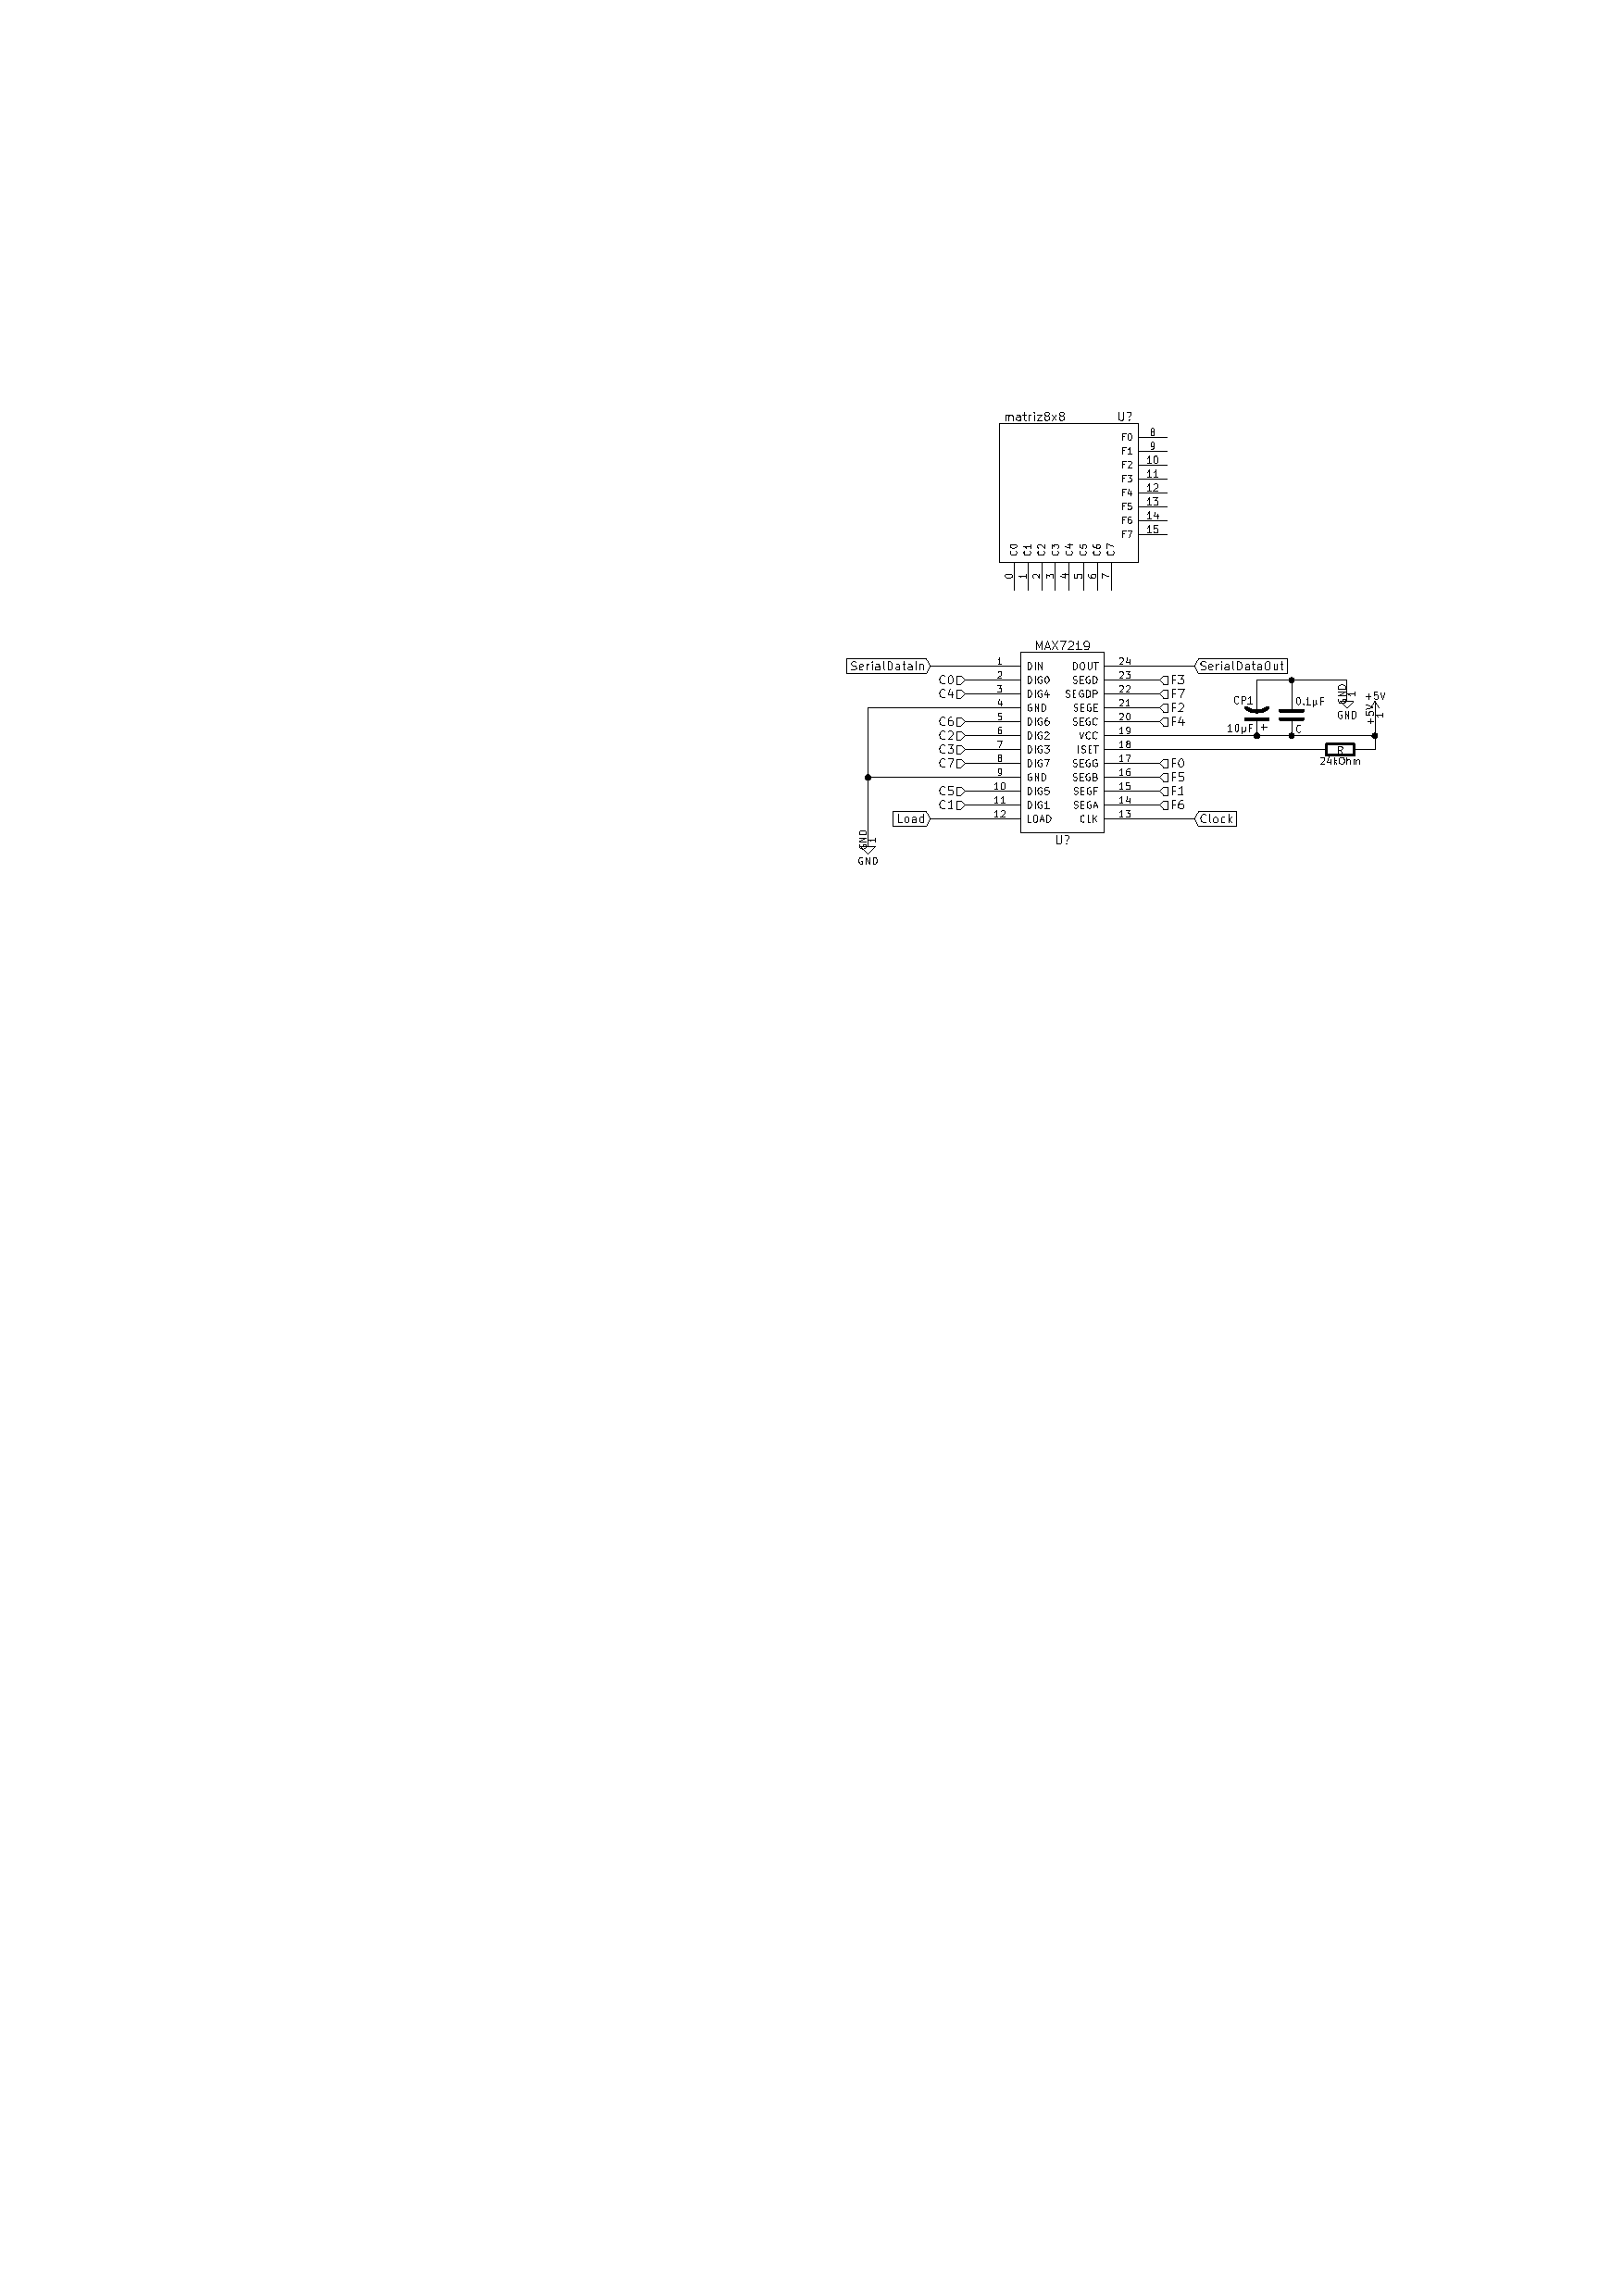
\includegraphics[width=\textwidth]{imagenes/hw/moduloEsquematico}
		\caption{Esquema de conexiones de un módulo funcional.}
		\label{fig:hw-moduloEsquematico}
	\end{center}
\end{figure}

\begin{figure}[ht!]
	\begin{center}
		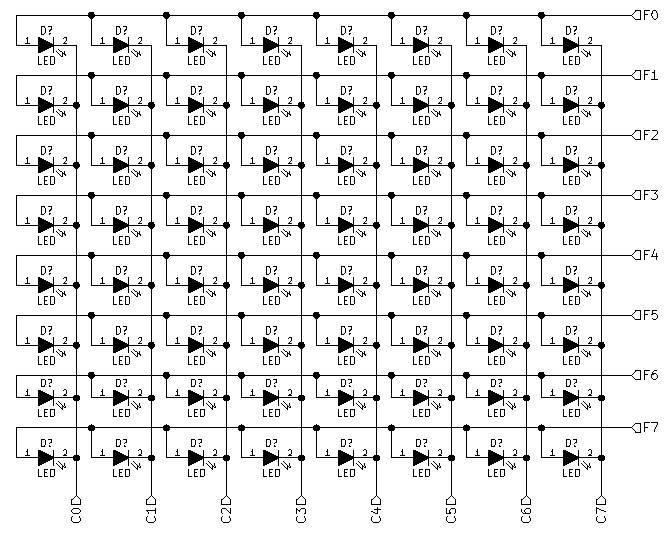
\includegraphics[width=0.8\textwidth]{imagenes/hw/moduloLED}
		\caption{Esquema de conexiones de la matriz de LEDs.}
		\label{fig:hw-moduloLED}
	\end{center}
\end{figure}

\begin{figure}[ht!]
	\begin{center}
		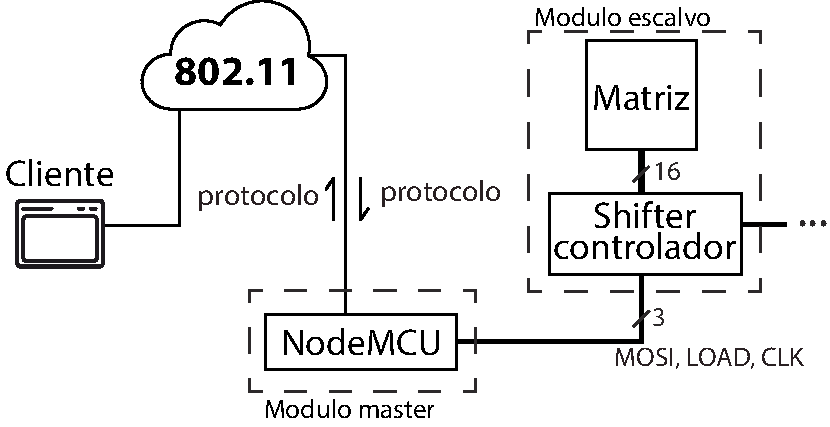
\includegraphics[width=0.9\textwidth]{imagenes/hw/diagrama-bloques-general}
		\caption{Esquema general entre todos los componentes del sistema.}
		\label{fig:hw-diagrama-general}
	\end{center}
\end{figure}


El microcontrolador envía la información de a un byte por vez al primer shifter que esta conectado a través del pin \texttt{SerialDataIn} (pin 1, ver figura \ref{fig:hw-moduloEsquematico}), previamente seteando el pin \texttt{Load} en bajo y terminando la transmisión poniendo en alto. Luego de 16.5 ciclos el shifter retransmite a el esclavo más proximo, asi sucesivamente con los demás esclavos. 

El MAX7219 recibe una secuencia de bytes (desde otro esclavo o del master) por serie y los deriva a la columna que corresponda para cada instante en la matriz de LEDs de su modulo.

\section{Diseño de software}


\subsection{Panel de configuración}
El panel de configuración consiste en una aplicación multiplataforma de escritorio escrita en C++ utilizando el framework de desarrollo Qt, que tiene como objetivo conectarse con el módulo NodeMCU (ESP8266) presente en el cartel a través de una conexión TLS.

La aplicación inicia la conexión con el sistema y, una vez establecida, permite cambiar el mensaje a mostrar, recuperar el mensaje completo que se está mostrando actualmente, cambiar opciones de animación, y modificar la red a la cual el cartel se conectará la próxima vez que se reinicie.

En la figura \ref{fig:screenshot-panel} se observa una captura de pantalla de la aplicación de escritorio.

%%%
%	TODO: Sacar un screen shoot

% \begin{figure}[ht!]
% 	\begin{center}
% 		\centering
% 		\includegraphics[scale=0.8]{imagenes/screenshot-panel.png}
% 		\caption{Captura de pantalla de la aplicación de escritorio.}
% 		\label{fig:screenshot-panel}
% 	\end{center}
% \end{figure}

\subsection{Software embebido}


\section{Conclusiones}



\subsection{Cronograma}
Como se puede observar en el apartado de las conclusiones parciales, el desarrollo de las actividades viene cumpliendo satisfactoriamente con los tiempos del cronograma estipulado. En el cronograma presente de la figura \ref{fig:cronograma} se observa las actividades que quedan realizar. En principio no se realizará ninguna corrección en cuanto al tiempo estipulado de las tareas que quedan por completar.

\begin{figure}[h!]
    \centering
    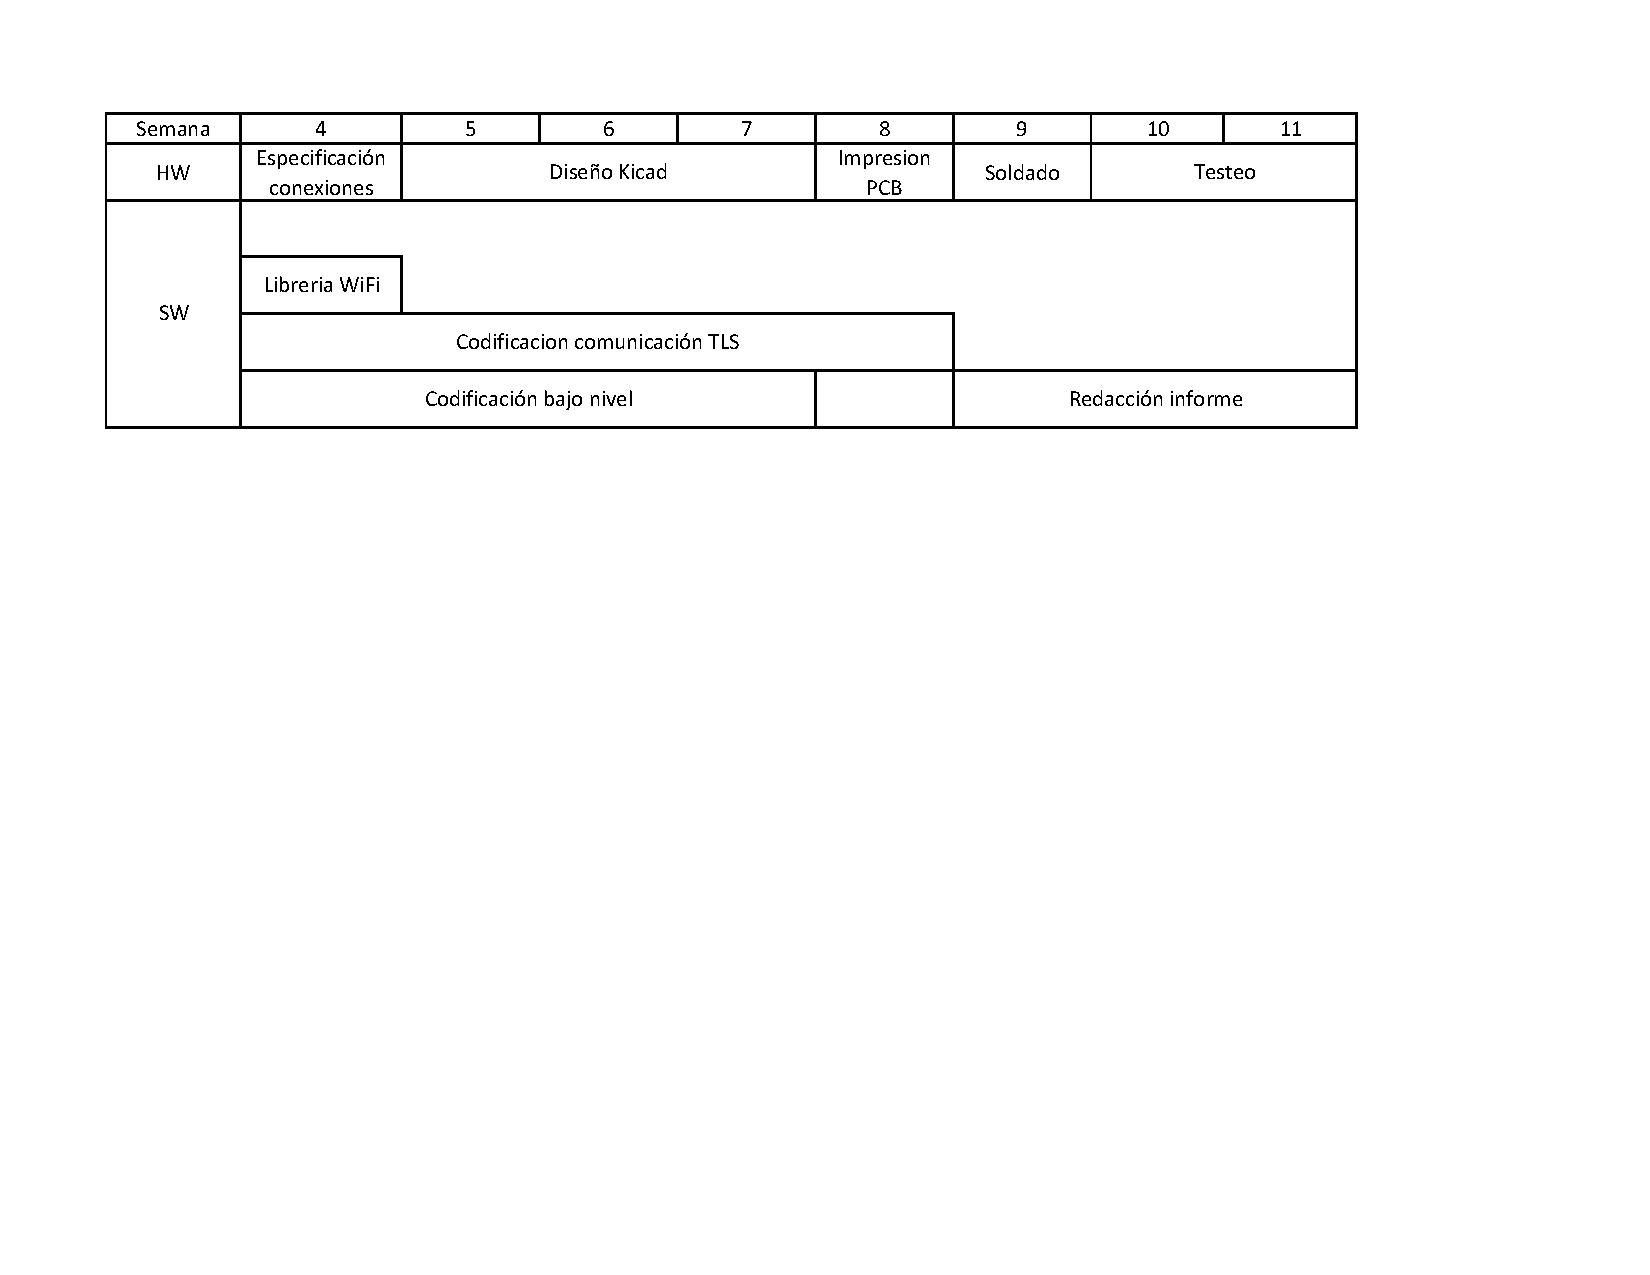
\includegraphics[width=\linewidth]{imagenes/cronograma.pdf}
    \caption{Cronograma de las semanas restantes.}
    \label{fig:cronograma}
\end{figure}

\subsection{Presupuesto}
En cuanto al presupuesto los precios son estimativos y en pesos. En el presupuesto no se tienen en cuenta los componentes varios (cables, gabinete, estaño, etc), ni el costo de impresión en el papel fotográfico para el PCB.

	\begin{table}[ht]
		\centering
		\caption{Presupuesto tentativo módulo Master. (Cantidades en ARS)}
	\begin{spreadtab}{{tabular}{cccc}}
		@ Item							& @ Unidades& @ Precio unidad (\$)	& @ Subtotal (\$)\\ \hline
		@ NodeMCU Esp8266				& 1			& :={200}				& b2*c2		\\
		@ PCB							& 1			& :={100}				& b3*c3		\\
		@ Transistor NPN\footnotemark	& 3	& :={4}	& b4*c4		\\
		@ Resistencia 56KOhm			& 3			& :={1}					& b5*c5		\\
		@ Resistencia 680Ohm			& 3			& :={1}					& b6*c6		\\
		@ Jumpers						& 4			& :={1}					& b7*c7		\\
		@ Jack con bornera				& 1			& :={20}				& b8*c8		\\
		@ Pulsador						& 1			& :={20}				& b9*c9		\\
		@ Tecla Rocker Switch 			& 1			& :={30}				& b10*c10	\\
		@ Regleta de 1x15 pines hembra	& 2			& :={7}					& b11*c11	\\
		@ Hoja A4 fotográfico			& 1			& :={20}				& b12*c12	\\\hline
		@ Total							& 			&						& \$ :={sum(d2:d12)}\\ \hline
	\end{spreadtab}
	\end{table}

	\footnotetext{Del tipo 2n2222 o similar, para el testeo se utilizó el transistor 2n2369.}

	\begin{table}[ht]
		\centering
		\caption{Presupuesto tentativo módulo Esclavo. (Cantidades en ARS)}
	\begin{spreadtab}{{tabular}{cccc}}
		@ Item									& @ Unidades& @ Precio unidad (\$)	& @ Subtotal (\$)\\ \hline
		@ LED									& 64		& :={1}					& b2*c2		\\
		@ PCB									& 1			& :={100}				& b3*c3		\\
		@ MAX7219								& 1			& :={45}				& b4*c4		\\
		@ Capacitor Polarizado	10µF			& 1			& :={3}					& b5*c5		\\
		@ Capacitor no polarizado 0.1µF			& 1			& :={3}					& b6*c6		\\
		@ Resistencia 24KOhm					& 1			& :={1}					& b7*c7		\\
		@ Conector hembra 8 Pin	(25.4mm)		& 2			& :={15}				& b8*c8		\\
		@ Conector hembra 5 Pin	(25.4mm)		& 2			& :={10}				& b9*c9		\\
		@ Regleta de 1x12 pines hembra (1.27mm)	& 2			& :={7}					& b10*c10	\\
		@ Hoja A4 fotográfico					& 1			& :={20}				& b11*c11	\\\hline
		@ Total									& 			&						& \$ :={sum(d2:d11)}\\ \hline
	\end{spreadtab}
	\end{table}